\documentclass[a4paper,11pt]{article}
\usepackage[T1]{fontenc}
\usepackage[utf8]{inputenc}
\usepackage{lmodern} 
\usepackage[portuguese]{babel}
\usepackage{graphicx}			%para imagens
\usepackage{epstopdf} 			%resolve problemas eps-pdf
\usepackage{fancyhdr}			% para o cabeçalho bonito
\usepackage{caption}				%para legendas
\usepackage{subcaption}			% e sublegendas
\usepackage{placeins} 			%controlar o lugar dos floats
\pagestyle{fancy} 				% número de pag e cabeçalho
\usepackage{slashbox} 			% criando caixas maneiras
\usepackage{wrapfig} 			%texto em volta da imagem
\usepackage{txfonts} 			%fontes bonitas? acho que para o título
\usepackage[usenames]{color} 	% algo com gunplot e eps
\graphicspath{{./images/}{./graph/}}		% procura imagens nessa pasta
\usepackage{epsf} 			%%para colocar .ps 


\newcommand{\HRule}{\rule{\linewidth}{0.5mm}}


%@@@@@@@@@@@@@@@@      Cabeçalho de cada página      @@@@@@@@@@@@@@@@@@@@@@

\setlength{\headheight}{15pt}%compila sem erro
	\fancyhead{}
	\fancyfoot{}
	\fancyhead[R]{Física Experimental 4}%direito superior
	\fancyhead[L]{\includegraphics[height=0.25in]{./images/logo_unb.pdf}}%esquerda superior
	\fancyfoot[C]{\thepage}%baixo centro
%E: Even page, O: Odd page, L: Left field, C: Center field, R: Right field, H: Header, F: Footer
% em documentos com dois lados use LO, RO. como esse documento não tem lados essa opção é inútil


\begin{document}
\begin{titlepage}
\begin{center}

% Upper part of the page. The '~' is needed because \\
% only works if a paragraph has started.
\includegraphics[width=\textwidth]{logo_unb.pdf}~\\[1cm]

\Huge Física Experimental 4\\[0.5cm]

\huge Experimento IV

% Title
\HRule \\[0.4cm]
{ \huge \bfseries  Interferômetro de Michelson}\\[0.4cm]

\HRule \\[0.5cm]

{\large \today}


\vfill %%o que vier depois vai ao fim da páginda


% Author and supervisor

	\begin{center} \large
		\begin{tabular}{llr} \
		& & \\[0.05cm]		
		Professora & Nadia Maria de Liz Koche & \\
		
		Alunos:& & \\
		& Juarez A.S.F 					& 11/0032829\\
		& Sérgio Fernandes da Silva Reis & 11/0140257\\
		& Jedhai Pimentel				& 09/0007883\\	[0.05cm]	
		\end{tabular}

	
	\end{center}


\end{center}
\end{titlepage}



\tableofcontents

\newpage

%@@@@@@@@@@@@@@@@@@@@@@@@@@@@@@@@@@@@@@@@@@@@@@@@@@@@@@@@@@@
%@@@@@@@@@@@@@@@@      OBJETIVOS      @@@@@@@@@@@@@@@@@@@@@@
%@@@@@@@@@@@@@@@@@@@@@@@@@@@@@@@@@@@@@@@@@@@@@@@@@@@@@@@@@@@
\section{Objetivos}
\paragraph{} Este experimento objetiva verificar a lei de Malus, verificar o estado de polarização da luz que passa por uma placa de \Large $ \frac{\lambda}{4} $ \normalsize e determinar  aproximadamente o índice de refração de um filtro de vidro.

%@@@@@@@@@@@@@@@@@@@@@@@@@@@@@@@@@@@@@@@@@@@@@@@@@@@@@@@@@@@
%@@@@@@@@@@@@@@@        MATERIAIS         @@@@@@@@@@@@@@@@@@
%@@@@@@@@@@@@@@@@@@@@@@@@@@@@@@@@@@@@@@@@@@@@@@@@@@@@@@@@@@@
\section{Materiais}
\paragraph{} Este experimento fez uso de:
\begin{itemize}
	\item[•]Banco ótico
	\item[•]Lampada fixa em \emph{Housing} contendo lente colimadora
	\item[•]Fonte de alimentação para lâmpada
	\item[•]2 Polarizadores rotativos com marcação em grau[$ \pm 0.5 º $]
	\item[•]Placa de um quarto de onda
	\item[•]Luxímetro digital[$ \pm $ max(1 , 5\% da medida)] 
	\item[•]Filtro absolvedor de infravermelho
	\item[•]Filtro absolvedor de vermelho
	\item[•]Régua milimetrada[$ \pm $ 0.5 mm]
	\item[•]espectroscópio com montagem de lâmpada de 6V e filtro de vidro
\end{itemize}
\newpage
%@@@@@@@@@@@@@@@@@@@@@@@@@@@@@@@@@@@@@@@@@@@@@@@@@@@@@@@@@@@
%@@@@@@@@@@@@@@        INTRODUCAO       @@@@@@@@@@@@@@@@@@@@
%@@@@@@@@@@@@@@@@@@@@@@@@@@@@@@@@@@@@@@@@@@@@@@@@@@@@@@@@@@@

\section{Introdução}
\paragraph{} Dizemos que uma onda eletromagnética é orientada pelo plano que contem a direção de perturbação do campo elétrico e a direção de propagação da onda. Podemos classificar uma luz ou uma onda eletromagnéticas em geral observando esses planos orientadores para as diversas frentes de onda que compões o feixe de luz. No caso de serem todos paralelos entre si dizemos que a luz é polarizada, caso contrário ela será não-polarizada. Materiais polarizadores são aqueles que permitem passar apenas ondas com uma dada orientação. A polarização pode se dar de duas formas.

\paragraph{} A primeira é a polarização por absorvição, ela ocorre quando as moléculas do material estão dispostas de forma a serem capazes de absorver a componente do campo elétrico em uma certa orientação $\vec{a}$.A direção de polarização $\vec{p}$ é aquela perpendicular à $\vec{a}$ pois somente a componente na direção $\vec{p}$ de uma onda passará pelo material\footnote{$\vec{a}$ de absorvição e $\vec{p}$ de polarização}. A figura \ref{fig:pol-linear} ilustra essa polarização linear. Para sabermos a intensidade de radiação linearmente polarizada na direção $\vec{u}$ que passará por um polarizador devemos achar a componente do campo elétrico na direção $\vec{p}$. Como a intensidade da radiação $ I $ é proporcional ao quadrado do campo elétrico temos a relação:
\begin{equation}
\begin{array}{lcc}
	I \quad \alpha \quad E_m^2  & \rightarrow & I = I_m \cos ^2 \theta
\end{array}	
\label{eq:Malus}
\end{equation}
sendo $\theta$ o ângulo entre $\vec{u}$ e $\vec{p}$. A equação \ref{eq:Malus} é conhecida como a \emph{Lei de Malus}. Um caso interessante desse tipo de polarização ocorre em cristais anisotrópicos.

\paragraph{}Nesses materiais a velocidade de propagação de uma onda não é a mesma em todas as direções. Sejam $\vec{n}_{max}$ e $\vec{n}_{min}$ as direções de maior e menor velocidade de propagação respectivamente. Uma onda polarizada em $\vec{p}$ terá suas componentes em ambos as direções $\vec{n}$ aceleradas diferentemente, de forma que a componente em $\vec{n}_{max}$ se adianta em relação a componente em  $\vec{n}_{min}$. No caso da espessura do material ser suficiente para que esse avanço seja de um quarto do comprimento de onda original as duas ondas estarão defasadas de 90º. Uma placa com essa propriedade é chamada de placa de $\frac{\lambda}{4}$. As componentes nas direções $\vec{n}_{max}$ e $\vec{n}_{min}$ 	nessa situação podem ser descritas por:
\begin{equation}
	\begin{array}{rcl}
		E_{\vec{n}_{max}} & = & E_1 \cos (\omega t + \pi/2) \\
		E_{\vec{n}_{min}} & = & E_2 \cos (\omega t) \\
	\end{array}
\end{equation}
\paragraph{}Se $E_1 = E_2$ diremos que a onda foi circularmente polarizada e caso contrário, elipticamente polarizada. A figura (\ref{fig:pol-circular}) ilustra a decomposição da onda após a placa de $ \frac{\lambda}{4}$ para o caso circular. Os eixos de max e min estão indicados e vemos também o campo soma das duas componentes.

\paragraph{}Outro processo de polarização ocorre por reflexão. Quando uma luz não-polarizada atinge uma superfície refletora existe reflexão preferencial das ondas cujo campo elétrico oscila perpendicularmente ao plano de incidência(plano que contem o raio incidente, o refletido e a normal à superfície). Em geral o campo elétrico refletido é não polarizado e possui componentes paralelas e normais ao plano  de incidência. Existe um ângulo $\varphi$ no entanto no qual a luz refletida é completamente polarizada na direção perpendicular ao plano de incidência,este é conhecido como \emph{ângulo de Brewster}. Uma propriedade interessante é que quando ocorre da luz refletida ser linearmente polarizada o ângulo entre o raio refletido e o refratado é de 90º. A figura (\ref{fig:brewster}) ilustra o fato. Usando a lei de Snell para um raio que viaja em meio de índice de refração $n_1$ e incide em outro de índice $n_2$ é possível obter:

\begin{equation}
	\tan \varphi = \frac{n_2}{n_1}
	\label{eq:n-refrac}
\end{equation}  

\paragraph{}Conhecendo o índice de refração $n_1$ do meio essa relação pode ser usada para determinar o índice de refração $n_2$ do material. Basta procurar pelo ângulo $\varphi$ de incidência que produz um raio refletido totalmente polarizado.
\FloatBarrier
\begin{figure}[!htp]
	\centering	
	
	\begin{subfigure}[!htp]{0.3\textwidth}
		\includegraphics[scale= 0.4]{./images/linear-pol.jpg}
		\caption{Polarização linear}
		\label{fig:pol-linear}
	\end{subfigure} 
	
	\begin{subfigure}[!htp]{0.3\textwidth}
		%\centering
		\includegraphics[scale= 0.3]{./images/circ-polarizared.jpg}
		\caption{Polarização circular}
		\label{fig:pol-circular}
	\end{subfigure}  
	\hspace{2 cm}
	\begin{subfigure}[!htp]{0.3\textwidth}
		%\centering		
		\includegraphics[scale= 0.4]{./images/polarization-by-reflex.jpg}
		\caption{Polarização por reflexão}
		\label{fig:brewster}
	\end{subfigure}  
	\caption{Diferentes processos de polarização}
\end{figure}
\FloatBarrier

\newpage


%@@@@@@@@@@@@@@@@@@@@@@@@@@@@@@@@@@@@@@@@@@@@@@@@@@@@@@@@@@@
%@@@@@@@@@@@@       PROCEDIMENTOS        @@@@@@@@@@@@@@@@@@@
%@@@@@@@@@@@@@@@@@@@@@@@@@@@@@@@@@@@@@@@@@@@@@@@@@@@@@@@@@@@
\section{Procedimentos}
	\subsection*{1.Verificação da Lei de Malus}
		\paragraph{}Primeiramente montam-se os instrumentos a serem utilizados sobre o banco ótico como na figura \ref{fig:montage1}. A fonte é ligada e toma-se cuidado para regular a altura dos instrumentos óticos de forma que a luz no detector ocupe toda a área do sensor. A figura não ilustra mas o polarizador ajustável é colocado o mais próximo possível do detector. Observando-se a medida do detector e procura-se a posição angular do polarizador ajustável na qual a intensidade é máxima. O ângulo é então variado de 10º em 10º e as medidas observadas são anotadas até que se tenha andado 180º. Retira-se o filtro de infravermelho e as medidas são feitas novamente.
		
	\subsection*{2.Polarização circular elíptica}
		\paragraph{}Na mesma montagem do procedimento anterior ajusta-se o analisador(polarizador rotativo) na posição de mínima transmissão. Com essa regulagem os instrumentos são montados sobre o banco ótico como na figura \ref{fig:montagem2}. A placa de $\frac{\lambda}{4}$ é então girada até que a medida no sensor seja mínima. O estado de polarização é então analisado\footnote{Analisar o estado de polarização no nosso contexto é, como já foi feito no primeiro procedimento, fazer variar em 180º o ângulo do analisador de 10º em 10º anotando-se em cada etapa a medida no sensor.}. A placa de$\frac{\lambda}{4}$ é então girada da sua posição inicial em 90º e o estado de polarização é analisado. Com a placa de $\frac{\lambda}{4}$ nesse estado o analisador é colocado em 45º com o polarizador fixo e mais uma vez analisamos o estado de polarização. O filtro de vermelho é então retirado e as medidas refeitas.  
		
		
	\subsection*{3.Determinando índice de refração utilizando polarização por reflexão}
		\paragraph{}O experimento usa um espectroscópio e a montagem é representada simplificadamente na figura \ref{fig:montagem3}. Na figura o colimador está fixo, o telescópio é móvel e a placa de vidro encontra-se fixa à uma mesa com marcação em graus que pode girar. Tanto o movimento da mesa como o do telescópio são em torno do eixo da mesa. A fonte é ligada, a mesa é fixada e procura-se com o movimento do telescópio o feixe de luz refletido. Ajusta-se então o foco do colimador de forma que a imagem obtida seja nítida. Colocando-se um polarizador  entre a ocular do telescópio e o olho pode-se decidir se a luz refletida é polarizada ou não. Nosso objetivo é achar o ângulo $\alpha$ em que isso ocorre. Gira-se a mesa(modificando o ângulo com que a luz colimada incide na placa) e procura-se novamente com o telescópio a luz refletida. Observa-se a polarização ou não da luz e o processo é repetido\footnote{É claro que a busca por esse ângulo segue um algoritmo lógico: se a intensidade observada esta diminuindo estamos no caminho certo, caso contrários devemos ir na outra direção.} até que se ache o ângulo $\alpha$ procurado. Com esse ângulo a fórmula \ref{eq:Malus} pode ser usada para determinar o índice de refração $n_2$ do material supondo o índice de refração do ar $n_1 = 1$. 
		
\FloatBarrier
\begin{figure}
	\centering		
	\begin{subfigure}[!htp]{\textwidth}
		\centering
		\includegraphics[scale= 0.5]{./images/montagem1-1.jpg}
		\caption{Montagem 1}
		\label{fig:montage1}
	\end{subfigure}  
	
	\begin{subfigure}[!htp]{\textwidth}
		\centering		
		\includegraphics[scale= 0.5]{./images/montagem1-2.jpg}
		\caption{Montagem 2}
		\label{fig:montagem2}
	\end{subfigure}  

	\begin{subfigure}[!htp]{\textwidth}
		\centering		
		\includegraphics[scale= 0.7]{./images/montagem1-3.jpg}
		\caption{Montagem 3}
		\label{fig:montagem3}
	\end{subfigure}  
	\caption{Procedimentos}
\end{figure}
\FloatBarrier

%@@@@@@@@@@@@@@@@@@@@@@@@@@@@@@@@@@@@@@@@@@@@@@@@@@@@@@@@@@@
%@@@@@@@@@@@@@@@@@@@       DADOS      @@@@@@@@@@@@@@@@@@@@@@
%@@@@@@@@@@@@@@@@@@@@@@@@@@@@@@@@@@@@@@@@@@@@@@@@@@@@@@@@@@@

\section{Dados}
\paragraph{} Os resultados do procedimento 1 são mostrados na tabela \ref{tab:proced1}. A segunda coluna mostra os dados da análise de polarização quando usamos o filtro de infravermelho e a terceira os dados quando removemos o filtro. Os resultados do procedimento 2 são vistos na tabela \ref{tab:proced2}. A segunda coluna  nos mostra o estado de polarização quando a placa de $\frac{\lambda}{4}$ é colocada de forma que a intensidade seja mínima, na terceira coluna a placa foi girada em 90º e na quarta temos o estado de polarização com o polarizador fixo em 45º. A tabela \ref{tab:proced3} mostra os dados das medidas com placa de $\frac{\lambda}{4}$ mas sem o filtro de vermelho. Os dados das três tabelas são plotados nos gráficos \ref{graph:4-1}, \ref{graph:4-2} e \ref{graph:4-3}.

\begin{table}[!htp]
	\hspace{-1.5 cm}
	\begin{minipage}{0.4\textwidth}
			\begin{tabular}{|c|c|c|} \hline
				$\theta \pm 0.5º$ & c/ filtro & sem filtro \\ \hline
						 0.0 & 260 & 735\\ \hline 
		 10.0 & 253 & 680 \\ \hline 
		 20.0 & 235 & 610 \\ \hline 
		 30.0 & 212 & 520 \\ \hline 
		 40.0 & 167 & 410 \\ \hline 
		 50.0 & 128 & 300 \\ \hline 
		 60.0 & 92 & 205 \\ \hline 
		 70.0 & 56& 130 \\ \hline 
		 80.0 & 28 & 92 \\ \hline 
		 90.0 & 14 & 91\\ \hline 
		 100.0 & 16 & 120 \\ \hline 
		 110.0 & 30 & 203 \\ \hline 
		 120.0 & 59& 296\\ \hline 
		 130.0 & 92 & 415 \\ \hline 
		 140.0 & 132& 540 \\ \hline 
		 150.0 & 172 & 635 \\ \hline 
		 160.0 & 210& 720\\ \hline 
		 170.0 & 230 & 760\\ \hline 
		 180.0 & 255 & 770 \\ \hline 
		 180.0 & 255& 770 \\ \hline 

			\end{tabular}
			\caption{Procedimento 1}	
			\label{tab:proced1}
	\end{minipage}
	\hspace{1.5 cm}
	\begin{minipage}{0.4\textwidth}
			\begin{tabular}{|c|c|c|c|}\hline
			$\theta \pm 0.5º$ & $\frac{\lambda}{4}$ em 0º &$\frac{\lambda}{4}$ em 90º & Polarizador em 45º  \\ \hline
					 0.0 & 35 & 36 & 16 \\ \hline 
		 10.0 & 33 & 35 & 15 \\ \hline 
		 20.0 & 30 & 32 & 14 \\ \hline 
		 30.0 & 26 & 28 & 14 \\ \hline 
		 40.0 & 20 & 22 & 15 \\ \hline 
		 50.0 & 14 & 16 & 16 \\ \hline 
		 60.0 & 10 & 11 & 17 \\ \hline 
		 70.0 & 5& 6 & 18 \\ \hline 
		 80.0 & 2& 3 & 19 \\ \hline 
		 90.0 & 1& 1 & 20 \\ \hline 
		 100.0 & 3 & 3 & 20 \\ \hline 
		 110.0 & 8 & 7 & 21 \\ \hline 
		 120.0 & 14 & 12 & 20 \\ \hline 
		 130.0 & 20 & 18 & 20 \\ \hline 
		 140.0 & 25 & 24 & 19 \\ \hline 
		 150.0 & 31 & 30 & 18 \\ \hline 
		 160.0 & 35 & 33 & 17 \\ \hline 
		 170.0 & 36 & 35 & 16 \\ \hline 
		 180.0 & 36 & 35 & 16 \\ \hline 
		 180.0 & 36 & 35 & 16 \\ \hline 

			\end{tabular}
			\caption{Procedimento 2}
			\label{tab:proced2}
	\end{minipage}
	
	\caption*{}
\end{table}
\FloatBarrier
\begin{table}[!t]
	\vspace{-2.5 cm}
			\centering
			\begin{tabular}{|c|c|c|c|}\hline
			$\theta \pm 0.5º$ & $\frac{\lambda}{4}$ em 0º &$\frac{\lambda}{4}$ em 90º & Polarizador em 45º  \\ \hline
					 0.0 & 425 & 430 & 247\\ \hline 
		 10.0 & 414 & 419 & 243 \\ \hline 
		 20.0 & 396 & 398 & 241 \\ \hline 
		 30.0 & 342 & 357 & 245 \\ \hline 
		 40.0 & 283 & 288 & 249 \\ \hline 
		 50.0 & 207 & 215 & 245 \\ \hline 
		 60.0 & 145 & 159 & 250 \\ \hline 
		 70.0 & 83 & 90 & 250 \\ \hline 
		 80.0 & 42 & 44 & 254 \\ \hline 
		 90.0 & 23 & 25 & 250 \\ \hline 
		 100.0 & 26 & 23 & 245 \\ \hline 
		 110.0 & 51 & 44 & 246 \\ \hline 
		 120.0 & 93 & 89 & 248 \\ \hline 
		 130.0 & 155 & 146 & 247 \\ \hline 
		 140.0 & 221 & 208 & 241 \\ \hline 
		 150.0 & 293 & 277 & 243 \\ \hline 
		 160.0 & 350 & 342 & 243 \\ \hline 
		 170.0 & 393 & 393 & 241 \\ \hline 
		 180.0 & 405 & 409 & 240 \\ \hline 
		 180.0 & 405 & 409 & 240 \\ \hline 

			\end{tabular}
			\caption{Sem filtro vermelho}
			\label{tab:proced3}
\end{table}
\FloatBarrier

\FloatBarrier
\begin{figure}[!t]
\vspace{-2 cm}
\begin{minipage}{\textwidth}
					\centering
					\input{./graph/4-1.tex}  
					\caption{dados do experimento 1}
					\label{graph:4-1}
			
\end{minipage}
\vspace{1.0 cm}
\begin{minipage}{\textwidth}
					% GNUPLOT: LaTeX picture with Postscript
\begingroup
  \fontfamily{phv}%
  \selectfont
\definecolor{t}{rgb}{0.5,0.5,0.5}
  \makeatletter
  \providecommand\color[2][]{%
    \GenericError{(gnuplot) \space\space\space\@spaces}{%
      Package color not loaded in conjunction with
      terminal option `colourtext'%
    }{See the gnuplot documentation for explanation.%
    }{Either use 'blacktext' in gnuplot or load the package
      color.sty in LaTeX.}%
    \renewcommand\color[2][]{}%
  }%
  \providecommand\includegraphics[2][]{%
    \GenericError{(gnuplot) \space\space\space\@spaces}{%
      Package graphicx or graphics not loaded%
    }{See the gnuplot documentation for explanation.%
    }{The gnuplot epslatex terminal needs graphicx.sty or graphics.sty.}%
    \renewcommand\includegraphics[2][]{}%
  }%
  \providecommand\rotatebox[2]{#2}%
  \@ifundefined{ifGPcolor}{%
    \newif\ifGPcolor
    \GPcolortrue
  }{}%
  \@ifundefined{ifGPblacktext}{%
    \newif\ifGPblacktext
    \GPblacktextfalse
  }{}%
  % define a \g@addto@macro without @ in the name:
  \let\gplgaddtomacro\g@addto@macro
  % define empty templates for all commands taking text:
  \gdef\gplbacktext{}%
  \gdef\gplfronttext{}%
  \makeatother
  \ifGPblacktext
    % no textcolor at all
    \def\colorrgb#1{}%
    \def\colorgray#1{}%
  \else
    % gray or color?
    \ifGPcolor
      \def\colorrgb#1{\color[rgb]{#1}}%
      \def\colorgray#1{\color[gray]{#1}}%
      \expandafter\def\csname LTw\endcsname{\color{white}}%
      \expandafter\def\csname LTb\endcsname{\color{black}}%
      \expandafter\def\csname LTa\endcsname{\color{black}}%
      \expandafter\def\csname LT0\endcsname{\color[rgb]{1,0,0}}%
      \expandafter\def\csname LT1\endcsname{\color[rgb]{0,1,0}}%
      \expandafter\def\csname LT2\endcsname{\color[rgb]{0,0,1}}%
      \expandafter\def\csname LT3\endcsname{\color[rgb]{1,0,1}}%
      \expandafter\def\csname LT4\endcsname{\color[rgb]{0,1,1}}%
      \expandafter\def\csname LT5\endcsname{\color[rgb]{1,1,0}}%
      \expandafter\def\csname LT6\endcsname{\color[rgb]{0,0,0}}%
      \expandafter\def\csname LT7\endcsname{\color[rgb]{1,0.3,0}}%
      \expandafter\def\csname LT8\endcsname{\color[rgb]{0.5,0.5,0.5}}%
    \else
      % gray
      \def\colorrgb#1{\color{black}}%
      \def\colorgray#1{\color[gray]{#1}}%
      \expandafter\def\csname LTw\endcsname{\color{white}}%
      \expandafter\def\csname LTb\endcsname{\color{black}}%
      \expandafter\def\csname LTa\endcsname{\color{black}}%
      \expandafter\def\csname LT0\endcsname{\color{black}}%
      \expandafter\def\csname LT1\endcsname{\color{black}}%
      \expandafter\def\csname LT2\endcsname{\color{black}}%
      \expandafter\def\csname LT3\endcsname{\color{black}}%
      \expandafter\def\csname LT4\endcsname{\color{black}}%
      \expandafter\def\csname LT5\endcsname{\color{black}}%
      \expandafter\def\csname LT6\endcsname{\color{black}}%
      \expandafter\def\csname LT7\endcsname{\color{black}}%
      \expandafter\def\csname LT8\endcsname{\color{black}}%
    \fi
  \fi
  \setlength{\unitlength}{0.0500bp}%
  \begin{picture}(5668.00,3968.00)%
    \gplgaddtomacro\gplbacktext{%
      \csname LTb\endcsname%
      \put(774,576){\makebox(0,0)[r]{\strut{} 0}}%
      \put(774,861){\makebox(0,0)[r]{\strut{} 10}}%
      \put(774,1146){\makebox(0,0)[r]{\strut{} 20}}%
      \put(774,1431){\makebox(0,0)[r]{\strut{} 30}}%
      \put(774,1716){\makebox(0,0)[r]{\strut{} 40}}%
      \put(774,2002){\makebox(0,0)[r]{\strut{} 50}}%
      \put(774,2287){\makebox(0,0)[r]{\strut{} 60}}%
      \put(774,2572){\makebox(0,0)[r]{\strut{} 70}}%
      \put(774,2857){\makebox(0,0)[r]{\strut{} 80}}%
      \put(774,3142){\makebox(0,0)[r]{\strut{} 90}}%
      \put(774,3427){\makebox(0,0)[r]{\strut{} 100}}%
      \put(882,396){\makebox(0,0){\strut{} 3.5}}%
      \put(1774,396){\makebox(0,0){\strut{} 3.6}}%
      \put(2666,396){\makebox(0,0){\strut{} 3.7}}%
      \put(3559,396){\makebox(0,0){\strut{} 3.8}}%
      \put(4451,396){\makebox(0,0){\strut{} 3.9}}%
      \put(5343,396){\makebox(0,0){\strut{} 4}}%
      \put(144,2001){\makebox(0,0){\strut{}$k$}}%
      \put(3112,126){\makebox(0,0){\strut{}$\lambda$}}%
      \put(3112,3697){\makebox(0,0){\strut{}k vs. $\lambda$ : altos períodos}}%
    }%
    \gplgaddtomacro\gplfronttext{%
    }%
    \gplbacktext
    \put(0,0){\includegraphics{4-2}}%
    \gplfronttext
  \end{picture}%
\endgroup
  
					\caption{dados do experimento 2}
					\label{graph:4-2}
\end{minipage}
\end{figure}
\FloatBarrier

\FloatBarrier
\begin{figure}[!htp]

					% GNUPLOT: LaTeX picture with Postscript
\begingroup
  \fontfamily{phv}%
  \selectfont
\definecolor{t}{rgb}{0.5,0.5,0.5}
  \makeatletter
  \providecommand\color[2][]{%
    \GenericError{(gnuplot) \space\space\space\@spaces}{%
      Package color not loaded in conjunction with
      terminal option `colourtext'%
    }{See the gnuplot documentation for explanation.%
    }{Either use 'blacktext' in gnuplot or load the package
      color.sty in LaTeX.}%
    \renewcommand\color[2][]{}%
  }%
  \providecommand\includegraphics[2][]{%
    \GenericError{(gnuplot) \space\space\space\@spaces}{%
      Package graphicx or graphics not loaded%
    }{See the gnuplot documentation for explanation.%
    }{The gnuplot epslatex terminal needs graphicx.sty or graphics.sty.}%
    \renewcommand\includegraphics[2][]{}%
  }%
  \providecommand\rotatebox[2]{#2}%
  \@ifundefined{ifGPcolor}{%
    \newif\ifGPcolor
    \GPcolortrue
  }{}%
  \@ifundefined{ifGPblacktext}{%
    \newif\ifGPblacktext
    \GPblacktextfalse
  }{}%
  % define a \g@addto@macro without @ in the name:
  \let\gplgaddtomacro\g@addto@macro
  % define empty templates for all commands taking text:
  \gdef\gplbacktext{}%
  \gdef\gplfronttext{}%
  \makeatother
  \ifGPblacktext
    % no textcolor at all
    \def\colorrgb#1{}%
    \def\colorgray#1{}%
  \else
    % gray or color?
    \ifGPcolor
      \def\colorrgb#1{\color[rgb]{#1}}%
      \def\colorgray#1{\color[gray]{#1}}%
      \expandafter\def\csname LTw\endcsname{\color{white}}%
      \expandafter\def\csname LTb\endcsname{\color{black}}%
      \expandafter\def\csname LTa\endcsname{\color{black}}%
      \expandafter\def\csname LT0\endcsname{\color[rgb]{1,0,0}}%
      \expandafter\def\csname LT1\endcsname{\color[rgb]{0,1,0}}%
      \expandafter\def\csname LT2\endcsname{\color[rgb]{0,0,1}}%
      \expandafter\def\csname LT3\endcsname{\color[rgb]{1,0,1}}%
      \expandafter\def\csname LT4\endcsname{\color[rgb]{0,1,1}}%
      \expandafter\def\csname LT5\endcsname{\color[rgb]{1,1,0}}%
      \expandafter\def\csname LT6\endcsname{\color[rgb]{0,0,0}}%
      \expandafter\def\csname LT7\endcsname{\color[rgb]{1,0.3,0}}%
      \expandafter\def\csname LT8\endcsname{\color[rgb]{0.5,0.5,0.5}}%
    \else
      % gray
      \def\colorrgb#1{\color{black}}%
      \def\colorgray#1{\color[gray]{#1}}%
      \expandafter\def\csname LTw\endcsname{\color{white}}%
      \expandafter\def\csname LTb\endcsname{\color{black}}%
      \expandafter\def\csname LTa\endcsname{\color{black}}%
      \expandafter\def\csname LT0\endcsname{\color{black}}%
      \expandafter\def\csname LT1\endcsname{\color{black}}%
      \expandafter\def\csname LT2\endcsname{\color{black}}%
      \expandafter\def\csname LT3\endcsname{\color{black}}%
      \expandafter\def\csname LT4\endcsname{\color{black}}%
      \expandafter\def\csname LT5\endcsname{\color{black}}%
      \expandafter\def\csname LT6\endcsname{\color{black}}%
      \expandafter\def\csname LT7\endcsname{\color{black}}%
      \expandafter\def\csname LT8\endcsname{\color{black}}%
    \fi
  \fi
  \setlength{\unitlength}{0.0500bp}%
  \begin{picture}(6802.00,4534.00)%
    \gplgaddtomacro\gplbacktext{%
      \csname LTb\endcsname%
      \put(774,576){\makebox(0,0)[r]{\strut{} 0}}%
      \put(774,1146){\makebox(0,0)[r]{\strut{} 20}}%
      \put(774,1715){\makebox(0,0)[r]{\strut{} 40}}%
      \put(774,2285){\makebox(0,0)[r]{\strut{} 60}}%
      \put(774,2854){\makebox(0,0)[r]{\strut{} 80}}%
      \put(774,3424){\makebox(0,0)[r]{\strut{} 100}}%
      \put(774,3993){\makebox(0,0)[r]{\strut{} 120}}%
      \put(1339,396){\makebox(0,0){\strut{} 10}}%
      \put(1910,396){\makebox(0,0){\strut{} 20}}%
      \put(2481,396){\makebox(0,0){\strut{} 30}}%
      \put(3051,396){\makebox(0,0){\strut{} 40}}%
      \put(3622,396){\makebox(0,0){\strut{} 50}}%
      \put(4193,396){\makebox(0,0){\strut{} 60}}%
      \put(4764,396){\makebox(0,0){\strut{} 70}}%
      \put(5335,396){\makebox(0,0){\strut{} 80}}%
      \put(5906,396){\makebox(0,0){\strut{} 90}}%
      \put(6477,396){\makebox(0,0){\strut{} 100}}%
      \put(144,2284){\makebox(0,0){\strut{}f(k)}}%
      \put(3679,126){\makebox(0,0){\strut{}k}}%
      \put(3679,4263){\makebox(0,0){\strut{}Frequênia dos Períodos}}%
    }%
    \gplgaddtomacro\gplfronttext{%
    }%
    \gplbacktext
    \put(0,0){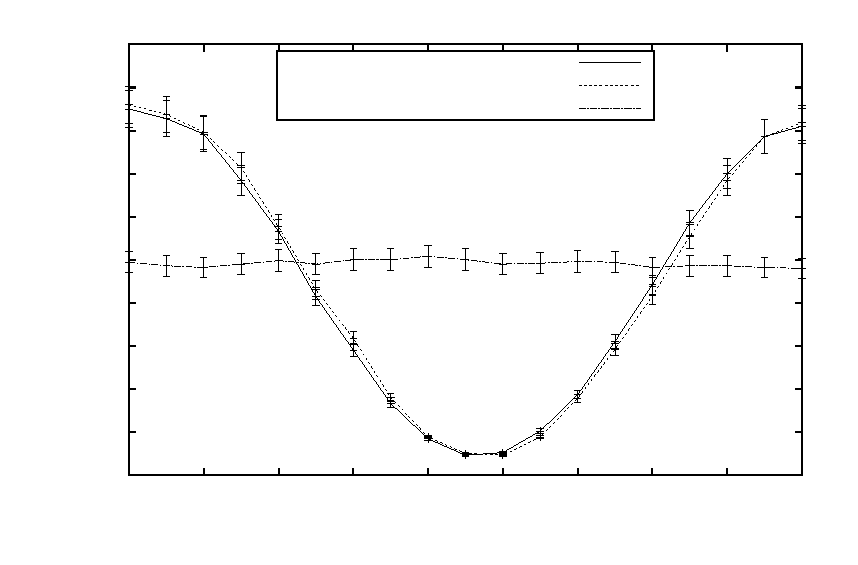
\includegraphics{4-3}}%
    \gplfronttext
  \end{picture}%
\endgroup
  
					\caption{experimento 2 sem filtro vermelho}
					\label{graph:4-3}

\end{figure}
\FloatBarrier

\paragraph{} O ângulo de Brewster achado para a placa de vidro no procedimento 3 é:
	\begin{equation}		
	\centering
		\begin{tabular}{|c|}\hline 
			$\alpha = 57.10º \pm 0.05º$  \\	\hline
		\end{tabular}
	\label{eq:alpha-brewstar}	
\end{equation}
%@@@@@@@@@@@@@@@@@@@@@@@@@@@@@@@@@@@@@@@@@@@@@@@@@@@@@@@@@@@
%@@@@@@@@@@@@@@       Análise         @@@@@@@@@@@@@@@@@@@@@@
%@@@@@@@@@@@@@@@@@@@@@@@@@@@@@@@@@@@@@@@@@@@@@@@@@@@@@@@@@@@

\section{Análise de Dados}
	
	\paragraph{}Nos gráficos \ref{graph:4-1-fitted} e \ref{graph:4-2-fitted} a seguir mostramos a regressão dos dados obtidos nos procedimentos 1 e 2.

\begin{figure}[!htp]
		\begin{minipage}{\textwidth}
					% GNUPLOT: LaTeX picture with Postscript
\begingroup
  \makeatletter
  \providecommand\color[2][]{%
    \GenericError{(gnuplot) \space\space\space\@spaces}{%
      Package color not loaded in conjunction with
      terminal option `colourtext'%
    }{See the gnuplot documentation for explanation.%
    }{Either use 'blacktext' in gnuplot or load the package
      color.sty in LaTeX.}%
    \renewcommand\color[2][]{}%
  }%
  \providecommand\includegraphics[2][]{%
    \GenericError{(gnuplot) \space\space\space\@spaces}{%
      Package graphicx or graphics not loaded%
    }{See the gnuplot documentation for explanation.%
    }{The gnuplot epslatex terminal needs graphicx.sty or graphics.sty.}%
    \renewcommand\includegraphics[2][]{}%
  }%
  \providecommand\rotatebox[2]{#2}%
  \@ifundefined{ifGPcolor}{%
    \newif\ifGPcolor
    \GPcolorfalse
  }{}%
  \@ifundefined{ifGPblacktext}{%
    \newif\ifGPblacktext
    \GPblacktexttrue
  }{}%
  % define a \g@addto@macro without @ in the name:
  \let\gplgaddtomacro\g@addto@macro
  % define empty templates for all commands taking text:
  \gdef\gplbacktext{}%
  \gdef\gplfronttext{}%
  \makeatother
  \ifGPblacktext
    % no textcolor at all
    \def\colorrgb#1{}%
    \def\colorgray#1{}%
  \else
    % gray or color?
    \ifGPcolor
      \def\colorrgb#1{\color[rgb]{#1}}%
      \def\colorgray#1{\color[gray]{#1}}%
      \expandafter\def\csname LTw\endcsname{\color{white}}%
      \expandafter\def\csname LTb\endcsname{\color{black}}%
      \expandafter\def\csname LTa\endcsname{\color{black}}%
      \expandafter\def\csname LT0\endcsname{\color[rgb]{1,0,0}}%
      \expandafter\def\csname LT1\endcsname{\color[rgb]{0,1,0}}%
      \expandafter\def\csname LT2\endcsname{\color[rgb]{0,0,1}}%
      \expandafter\def\csname LT3\endcsname{\color[rgb]{1,0,1}}%
      \expandafter\def\csname LT4\endcsname{\color[rgb]{0,1,1}}%
      \expandafter\def\csname LT5\endcsname{\color[rgb]{1,1,0}}%
      \expandafter\def\csname LT6\endcsname{\color[rgb]{0,0,0}}%
      \expandafter\def\csname LT7\endcsname{\color[rgb]{1,0.3,0}}%
      \expandafter\def\csname LT8\endcsname{\color[rgb]{0.5,0.5,0.5}}%
    \else
      % gray
      \def\colorrgb#1{\color{black}}%
      \def\colorgray#1{\color[gray]{#1}}%
      \expandafter\def\csname LTw\endcsname{\color{white}}%
      \expandafter\def\csname LTb\endcsname{\color{black}}%
      \expandafter\def\csname LTa\endcsname{\color{black}}%
      \expandafter\def\csname LT0\endcsname{\color{black}}%
      \expandafter\def\csname LT1\endcsname{\color{black}}%
      \expandafter\def\csname LT2\endcsname{\color{black}}%
      \expandafter\def\csname LT3\endcsname{\color{black}}%
      \expandafter\def\csname LT4\endcsname{\color{black}}%
      \expandafter\def\csname LT5\endcsname{\color{black}}%
      \expandafter\def\csname LT6\endcsname{\color{black}}%
      \expandafter\def\csname LT7\endcsname{\color{black}}%
      \expandafter\def\csname LT8\endcsname{\color{black}}%
    \fi
  \fi
  \setlength{\unitlength}{0.0500bp}%
  \begin{picture}(7936.00,5102.00)%
    \gplgaddtomacro\gplbacktext{%
      \csname LTb\endcsname%
      \put(946,704){\makebox(0,0)[r]{\strut{} 0}}%
      \put(946,1221){\makebox(0,0)[r]{\strut{} 100}}%
      \put(946,1737){\makebox(0,0)[r]{\strut{} 200}}%
      \put(946,2254){\makebox(0,0)[r]{\strut{} 300}}%
      \put(946,2771){\makebox(0,0)[r]{\strut{} 400}}%
      \put(946,3287){\makebox(0,0)[r]{\strut{} 500}}%
      \put(946,3804){\makebox(0,0)[r]{\strut{} 600}}%
      \put(946,4320){\makebox(0,0)[r]{\strut{} 700}}%
      \put(946,4837){\makebox(0,0)[r]{\strut{} 800}}%
      \put(1078,484){\makebox(0,0){\strut{} 0}}%
      \put(1796,484){\makebox(0,0){\strut{} 20}}%
      \put(2514,484){\makebox(0,0){\strut{} 40}}%
      \put(3232,484){\makebox(0,0){\strut{} 60}}%
      \put(3950,484){\makebox(0,0){\strut{} 80}}%
      \put(4667,484){\makebox(0,0){\strut{} 100}}%
      \put(5385,484){\makebox(0,0){\strut{} 120}}%
      \put(6103,484){\makebox(0,0){\strut{} 140}}%
      \put(6821,484){\makebox(0,0){\strut{} 160}}%
      \put(7539,484){\makebox(0,0){\strut{} 180}}%
      \put(176,2770){\rotatebox{-270}{\makebox(0,0){\strut{}luminosidade}}}%
      \put(4308,154){\makebox(0,0){\strut{}$\theta(º)$}}%
    }%
    \gplgaddtomacro\gplfronttext{%
      \csname LTb\endcsname%
      \put(4607,4664){\makebox(0,0)[r]{\strut{}com flitro}}%
      \csname LTb\endcsname%
      \put(4607,4444){\makebox(0,0)[r]{\strut{} sem filtro}}%
    }%
    \gplbacktext
    \put(0,0){\includegraphics{4-1-fitted}}%
    \gplfronttext
  \end{picture}%
\endgroup
  
					\caption{Regressão dos dado do experimento 1}
					\label{graph:4-1-fitted}
			
		\end{minipage}			
		\vspace{4 cm}
		\begin{minipage}{\textwidth}	
					\input{./graph/4-2-fitted.tex}  
					\caption{Regressão dos dado do experimento 2}
					\label{graph:4-2-fitted}
		\end{minipage}	
\end{figure}			


\paragraph{} No gráfico \ref{graph:4-1-fitted} as equações das curvas são:
\begin{equation}
	\begin{array}{cc}
		\mbox{ com filtro:} & 12.52  + 240.47 \cos^2(\frac{\pi(x - (4.73))}{180})
 \\
		\mbox{sem filtro:} & 81.49  + 668.99 \cos^2(\frac{\pi(x - (-5.50))}{180})
 \\		
	\end{array}
	\label{eq:preced1-malus}
\end{equation}

\paragraph{} No gráfico \ref{graph:4-2-fitted} as equações são:
\begin{equation}
	\begin{array}{cc}
		\mbox{ placa em 0º:} &  2.19  + 34.27 \cos^2(\frac{\pi(x - (-4.69))}{180})
 \\
		\mbox{ placa em 90º:} &  2.44  + 34.06 \cos^2(\frac{\pi(x - (-1.46))}{180})
 \\		
	\end{array}
	\label{eq:preced2-polarizacao-circ}
\end{equation}
\newpage

\subsection*{Procedimento I}
\paragraph{}Observa-se no gráfico \ref{graph:4-1-fitted} e nas equações \ref{eq:preced1-malus} o comportamento senoidal quadrático das curvas de intensidade luminosa como previsto por Malus. Notamos no entanto duas características que divergem do esperado. Primeiramente as medidas realizadas com filtro de infravermelho não foram capazes de eliminar a \emph{luminosidade de fundo} por completo. Apesar de termos obtido uma redução considerável no termo constante da fórmula não consegui-se obter um seno quadrado puro como previsto pela fórmula \ref{eq:Malus}. Em nossas medidas existem portanto comprimentos de onda que passam pelo filtro para os quais os polarizadores utilizados não funcionam apropriadamente. Além disso era esperado que com a introdução do filtro obtivéssemos apenas uma translação vertical dos dados e não é isso que se observa. Vemos que as amplitudes observadas variam cerca de 3 vezes.
\paragraph{}Alguns fatores, ou mais provavelmente, uma combinação de fatores podem ter contribuído para essas divergências entre os dados e a teoria. Analisando o estado de polarização da luz da fonte notamos que esta possui algum grau de polarização, o que certamente não bate com as condições da lei de Malus. Além disso notou-se que, medindo a intensidade captada tendo-se um polarizador fixo, não há uma posição angular do analisador que não diminua a intensidade observada. Ou seja, mesmo com os dois polarizadores em paralelo notamos uma queda no sinal. O analisador deve portanto absorver algum comprimento de onda, o que não era esperado. Apesar de tudo isso é sensato dizer que se observou no experimento uma luz linearmente polarizada.

\subsection*{Procedimento II}
\paragraph{} Primeiramente notemos as duas curvas próximas no gráfico \ref{graph:4-2-fitted} e as regressões em \ref{eq:preced2-polarizacao-circ}. Vemos que colocar a placa de $\frac{\lambda}{4}$ em uma posição de mínimo ou em posição perpendicular a esta primeira produz o mesmo resultado a menos de uma pequena constante de faze. Essa constante de faze pode ser explicada pela falta de precisão na marcação do ângulo de 90º. Dentro dessa faixa de erro podemos dizer que obtivemos o esperado teórico: colocar o campo paralelo a direção de $n_{max}$ ou de $n_{min}$ produz o mesmo resultado, a soma das componentes do campo em cada direção deve ser a mesma. 
\paragraph{}Vamos agora analisar o grau de elipticidade da polarização quando colocamos a placa de $\frac{\lambda}{4}$ em 45º com direção de polarização. Vê-se na figura \ref{fig:montagem2} que o vetores giram com amplitude variável formando uma elipse. Nota-se que os eixos da elipse são definidos pelas posições de máximo e mínimo(direções perpendiculares). Mediremos a elipticidade $\varepsilon$ procurando esses pontos de máximo e mínimo no gráfico \ref{graph:4-2} e na tabela \ref{tab:proced2}. Além disso lembramos que a intensidade medida é proporcional ao quadrado do campo, tiramos portanto a raiz quadrada de $I_{max}$ por $I_{min}$ para achar a elipticidade. Portanto:

\begin{displaymath}
	\begin{tabular}{c}
	$I_{max} = 21$ \\	
	$I_{min} = 14 $\\	
	$\varepsilon = \sqrt{\frac{I_{max}}{I_{min}}} = \sqrt{\frac{21}{14}}$ \\
\end{tabular}		
\end{displaymath}
\begin{equation}
	\varepsilon = 1.22
\end{equation}

\paragraph{}Notamos por último a importância do filtro vermelho. Ele reduz bastante a intensidade da radiação ao selecionar somente uma pequena faixa de comprimentos de onda. Sem ele não se veria as oscilações que ocorrem no sinal da placa de $\frac{\lambda}{4}$. É o que o ocorre em \ref{graph:4-3}. Poder-se-ia pensar que o sinal fora circularmente polarizado.

\subsection*{Procedimento III} 
\paragraph{}Tendo o ângulo de Brewstar em \ref{eq:alpha-brewstar} podemos usar a fórmula \ref{eq:n-refrac} para achar o índice de refração $n_{placa}$ da placa de vidro. Supomos para isso $n_{ar} = 1$

\begin{displaymath}
	n_{placa} = \tan(\alpha) \cdot n_{ar} = \tan{57.10} \cdot 1 
\end{displaymath}

\begin{equation}
	n_{placa} = 1.546
\end{equation}

\paragraph{}A tabela a seguir\footnote{Retirada de Halliday – Física – Vol. 4, 8a edição, página 18.
} relaciona o índice de refração de alguns materiais.
\FloatBarrier
\begin{figure}[!h]
\centering
	\includegraphics[scale=0.5]{indices-halliday.png}
	\caption{Índices de refração para alguns materiais}
\end{figure}
\FloatBarrier

\paragraph{}Comparando os índices vemos que o medido bate com índice de vidro de baixa dispersão.
%@@@@@@@@@@@@@@@@@@@@@@@@@@@@@@@@@@@@@@@@@@@@@@@@@@@@@@@@@@@
%@@@@@@@@@@@@@@       CONCLUSAO       @@@@@@@@@@@@@@@@@@@@@@
%@@@@@@@@@@@@@@@@@@@@@@@@@@@@@@@@@@@@@@@@@@@@@@@@@@@@@@@@@@@
\section{Conclusão}
\paragraph{}  A menos de alguns problemas discutidos na análise o experimento permitiu verificar a validade da lei de Malus e a influência dos filtros. Observou-se o estado elíptico produzido utilizando-se uma placa de $\frac{\lambda}{4}$  e foi possível medir a excentricidade desta polarização. Por fim calculou-se o índice de refração de uma placa de vidro usando o ângulo de Brewster e o obtido bateu com os valores tabelados. O experimento foi portanto bem sucedido.



%@@@@@@@@@@@@@@@@@@@@@@@@@@@@@@@@@@@@@@@@@@@@@@@@@@@@@@@@@@@
%@@@@@@@@@@@@@@       REFERÊNCIAS     @@@@@@@@@@@@@@@@@@@@@@
%@@@@@@@@@@@@@@@@@@@@@@@@@@@@@@@@@@@@@@@@@@@@@@@@@@@@@@@@@@@
\begin{thebibliography}{9}    
	 \bibitem{fis4}
  		JEWETT, J.W.; SERWAY, R.A.
  		\emph{Física para cientistas e engenheiros} volume 4 : Luz, Óptica e Física Moderna.
 		 8ª ed.
 		 São Paulo : Cengage Learning, 2012.
 		 
 	 \bibitem{fis4}
  		HALLIDAY, D.; RESNICK, R. ; WALKER.
  		\emph{Fundamentos de Física} volume 4
 		 8ª ed.
 		 Rio de Janeiro : LTC, 2009.
 		 
 	\bibitem{hyper-physis: pol by reflex}
 			R Nave. Polarization by Reflection. Disponível em: http://hyperphysics.phy-astr.gsu.edu/hbase/phyopt/polar. Acesso em: 3 de maio de 2013
 			 	
 	\bibitem{hyper-physis: pol classifi}
 			R Nave. Classification of Polarization . Disponível em: http://hyperphysics.phy-astr.gsu.edu/hbase/phyopt/polclas. Acesso em: 4 de maio de 2013


\end{thebibliography}



\end{document}
